\chapter{Local Flatness, Covariant Derivatives, and Curvature}

General relativity has the reputation of being very difficult, and Susskind begins by admitting that the reputation is not wholly undeserved. But the difficulty, at least at first, is not that the core ideas are inaccessible. It is that the subject is notationally heavy, calculationally intensive, and filled with indices that one must simply learn to carry. That is the spirit in which this chapter should be read. We will not try to hide the machinery before we understand what it is doing. These notes follow Leonard Susskind's lecture closely; where the blackboard itself carries mathematical content, we keep the supporting board evidence preserved through the work of LazyingArt LLC and Video2Book.

\section{Why We Need a Diagnostic for Curvature}

The lecture opens by lowering the temperature. There are elegant compact notations for general relativity, just as there are compact vector notations for Maxwell theory, but Susskind's point is that one does not really learn the subject by hiding the indices at the outset. He himself says that when he actually needs to calculate something, he returns to the same component language used here. So we begin without apology.

There is then a brief look outward. Current research ranges from quantum gravity and black-hole physics to numerical relativity, gravitational radiation, and even uses of the same equations in condensed matter and fluid dynamics. The digression is short, but it serves a purpose: the subject is alive. Then the lecture snaps back to the immediate course arc. Today is the last day of pure Riemannian geometry. Next time, geometry will become gravity.

The central question is therefore sharpened. How do we tell whether a gravitational field is real, as opposed to something produced by awkward coordinates? Susskind says that this is not merely similar to the problem of deciding whether a metric geometry is flat. It is the same problem.

So let us suppose we are handed a metric \(g_{mn}(x)\). We want a test for flatness that does not require guesswork about coordinates.

\paragraph{The bad way.} Search through all possible coordinate systems. Transform the metric into one trial coordinate system after another and keep asking whether, in some lucky frame, the components become those of a flat metric. This is hopeless. It is an infinite search.

\paragraph{The good way.} Construct a diagnostic quantity directly from the metric and its derivatives. Better still, make it a tensor. If a tensor vanishes in one coordinate system, it vanishes in all coordinate systems. Susskind even introduces the symbol \(R\) before telling us exactly how many indices it will carry. The target is already clear: we want an invariant object whose vanishing means flatness and whose nonvanishing signals genuine curvature.

That object will be the curvature tensor. But before it can be earned, the lecture deliberately backs up and rebuilds the minimum machinery that will make the construction intelligible.

\section{Metric Review: The Minimum Needed Machinery}

The lecture restarts from a very elementary place: we start with a space. The dimension can be anything, but one dimension is too simple to teach us much. A closed one-dimensional space is just a loop of some total length. A bug walking around it can count steps and measure that length, but if the rope is bent or wiggled in space without stretching, the intrinsic geometry is unchanged. In that sense one-dimensional geometry is characterized only by length.

Two dimensions are different. A plane, a sphere, the Earth's surface with mountains and valleys, a torus, or a surface with several holes are intrinsically different spaces. What characterizes them is the metric tensor.

The metric tells us the squared length of an infinitesimal displacement:
\begin{equation}
ds^2 = g_{mn}\,dx^m dx^n.
\end{equation}
Because \(ds^2\) is invariant, \(g_{mn}\) must transform as a tensor. This is not a decorative remark. It is exactly why the metric can encode intrinsic geometry rather than just coordinate bookkeeping.

The metric is also invertible:
\begin{equation}
g^{mr}g_{rn}=\delta^m{}_n.
\end{equation}
Here the Kronecker delta is written with one index up and one down, as a mixed tensor. The lecture pauses over this point because it is part of learning to read the index notation correctly.

In Riemannian geometry the metric is positive definite. Equivalently, for every nonzero displacement \(u^m\),
\begin{equation}
g_{mn}u^m u^n>0.
\end{equation}
Susskind phrases this geometrically: squared lengths are always positive. Later, when we pass from Riemannian to Einsteinian geometry, this will change.

The metric also raises and lowers indices:
\begin{align}
V_n &= g_{nm}V^m,\\
V^m &= g^{mn}V_n.
\end{align}
These are not two different vectors. They are the covariant and contravariant components of the same vector.

There is one more preliminary observation. If the components of the metric were constant in space, then one could always straighten out the coordinate axes and bring the metric into the form \(\delta_{mn}\). In that case the space would certainly be flat. So the real problem is not the existence of a metric, but its variation from point to point.

And here Susskind is careful about language. One should not say that a flat metric \emph{is} \(\delta_{mn}\). What is true is that in suitable coordinates a flat metric can be \emph{expressed} by the components \(\delta_{mn}\). In other coordinates the same flat geometry can look less simple. That distinction is going to matter immediately.

The question is now the one he asks explicitly on the board: to what extent can any metric be forced to look flat by a suitable choice of coordinates?

\section{Gaussian Normal Coordinates and Local Flatness}

Susskind answers that question with a local theorem. At any chosen point one can introduce coordinates, called Gaussian normal coordinates, in which the metric looks Euclidean and its first derivatives vanish. After shifting the chosen point to the origin, the board records the statement as
\begin{align}
g_{mn} &= \delta_{mn} \qquad \text{at } x=0,\\
\frac{\partial g_{mn}}{\partial x^r} &= 0 \qquad \text{at } x=0,\\
\frac{\partial^2 g_{mn}}{\partial x^r \partial x^s} &\neq 0
\qquad \text{in general.}
\end{align}

\begin{figure}[h]
\centering

\includegraphics[width=0.82\textwidth]{lecture_03_figure_03.png}
\caption{Gaussian normal metric conditions on the board, together with the partially visible quadratic coordinate expansion.}
\end{figure}

The lecture first explains this geometrically. We go to a point on a curved surface, draw coordinate axes there, and extend them as straight as possible. Later the phrase ``as straight as possible'' becomes geodesic language. For the moment the point is simpler: one can always flatten the metric to zeroth and first order at a point.

There is even some freedom left. If we have found one such local frame, we can rotate it and still keep \(g_{mn}=\delta_{mn}\) at the point. So Gaussian normal coordinates are not unique. What is unique is the local statement they make possible.

\subsection{Question \& Answer}

\paragraph{Question.} Is this simplification only at one point, or does it extend through a region?

\paragraph{Answer.} Only at the chosen point. One may build Gaussian normal coordinates at every point, but unless the space is truly flat, one cannot extend one such coordinate system throughout a region and keep all these simplifications. What survives away from the point are the second derivatives. Those cannot, in general, all be set to zero.

This is the first decisive step in the lecture. There is no invariant content in the statement that the metric is flat-looking at a point, or even flat-looking through first derivatives. That can always be arranged. So the real geometric information must live one order deeper.

Susskind then proves the local statement by counting parameters. Let the chosen point be the common origin of two coordinate systems \(x\) and \(y\), so that \(x=0\) and \(y=0\) refer to the same point. We expand the new coordinates in powers of the old ones:
\begin{equation}
x^m = y^m + C^m{}_{nr}\,y^n y^r + O(y^3).
\end{equation}
The board itself shows only the quadratic part,
\[
x^m = y^m + C^m{}_{nr}\,y^n y^r,
\]
and that is enough for the argument.

In four dimensions there are ten independent quadratic monomials \(y^n y^r\), because the product is symmetric in \(n\) and \(r\):
\begin{equation}
\#(y^n y^r)=\frac{4\cdot 5}{2}=10.
\end{equation}
For each upper index \(m\), there are therefore ten coefficients \(C^m{}_{nr}\), so altogether
\begin{equation}
\#(C^m{}_{nr})=4\times 10=40.
\end{equation}
On the other hand, a symmetric metric \(g_{mn}\) in four dimensions has ten independent components, and setting all first derivatives to zero gives four conditions for each component:
\begin{equation}
\#\bigl(\partial_r g_{mn}\bigr)=10\times 4=40.
\end{equation}
Forty unknown quadratic coefficients and forty first-derivative conditions: one can solve the equations to quadratic order. That is precisely what it means to make the metric equal to \(\delta_{mn}\) at the point and to kill all its first derivatives there.

But the freedom does not continue forever. At the next order the counting no longer works out in the same way. The second derivatives cannot, in general, all be removed. So it is exactly at second order that curvature begins to show itself.

This is why every smooth metric is locally flat and yet need not be globally flat. The statement is local, pointwise, and first-order. The real content of geometry survives beyond that.

\section{Why Ordinary Derivatives of Vector Components Fail}

Now the lecture explains why Gaussian normal coordinates were introduced in the first place. We want to differentiate vectors and tensors. But ordinary differentiation of components will not do.

Suppose we have a vector field, that is, a vector attached to every point. In flat Cartesian coordinates it is clear what it means for a vector at one point to be the same as a vector at a neighboring point: same direction, same length. In such a frame a constant vector field has constant components.

But now superimpose a curvilinear coordinate system on top of those locally straight coordinates. The vector may remain geometrically the same, yet its components in the curvilinear coordinates change from point to point, not because the vector has changed, but because the coordinate directions have changed.

\begin{figure}[h]
\centering

\includegraphics[width=0.9\textwidth]{lecture_03_figure_02.png}
\caption{Curved coordinates and the boxed zero-derivative condition. The board layout itself matters: quadratic coordinate transformation on the left, local sketch in the middle, boxed naive criterion on the right.}
\end{figure}

The board makes this point in three pieces at once. On the left, the earlier quadratic coordinate transformation is still visible:
\[
x^m = y^m + C^m{}_{nr}\,y^n y^r.
\]
In the middle, a local sketch compares a straight local frame with a curving coordinate line whose basis directions rotate from point to point. On the right, the lecture boxes the deliberately naive condition
\begin{equation}
\frac{\partial V_m}{\partial x^r}=0.
\end{equation}
The lower index on \(V_m\) is what the board visibly shows, and it is the safest figure-faithful transcription.

The point is not that this equation is meaningless. It is that it is not tensorial. It may hold in one coordinate system and fail in another.

\subsection{Question \& Answer}

\paragraph{Question.} Why can all these derivatives vanish in one coordinate system but not in another?

\paragraph{Answer.} Because the coordinates may be changing even when the vector is not. In a locally straight frame, a constant vector field can have constant components. In a curvilinear frame, the basis directions themselves rotate from point to point, so the components vary. The variation then belongs to the coordinates, not to the vector.

This is the first major conceptual obstacle of the lecture. If \(\partial_r V_m\) were the components of a tensor with indices \(m\) and \(r\), then once it vanished in one coordinate system it would vanish in all coordinate systems. Since that is not true, ordinary partial derivatives of vector components are not themselves tensor components.

\begin{figure}[h]
\centering
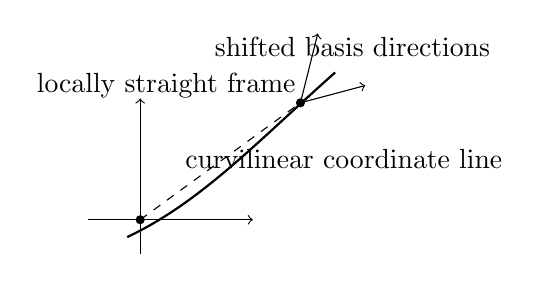
\begin{tikzpicture}[scale=1.1]
\draw[->] (-0.6,0) -- (1.3,0);
\draw[->] (0,-0.4) -- (0,1.4);
\fill (0,0) circle (1.5pt);
\draw[thick] (-0.15,-0.2) .. controls (0.7,0.2) and (1.35,0.9) .. (2.25,1.7);
\fill (1.85,1.35) circle (1.5pt);
\draw[->] (1.85,1.35) -- (2.6,1.55);
\draw[->] (1.85,1.35) -- (2.05,2.15);
\draw[dashed] (0,0) -- (1.85,1.35);
\node at (0.3,1.55) {locally straight frame};
\node at (2.35,0.7) {curvilinear coordinate line};
\node at (2.45,2.0) {shifted basis directions};
\end{tikzpicture}
\caption{Schematic reconstruction of the lecture's local comparison. The same geometric vector can acquire changing components because the coordinate frame itself changes from point to point.}
\end{figure}

So we are forced to a new question: can we define a derivative that agrees with ordinary differentiation in the nicest local frame, and yet remains a tensor when expressed in arbitrary coordinates?

\section{Covariant Derivative and the Christoffel Symbols}

Susskind introduces the covariant derivative operationally. To define the derivative of a vector at a point, we need only a small neighborhood of that point. So we first construct Gaussian normal coordinates there. In those coordinates the metric is as close to Cartesian as it can be, and at the chosen point its first derivatives vanish.

Now take a vector at a neighboring point and shift it back so that its tail sits at the base point, keeping its Gaussian-normal components fixed during that shift. Compare the shifted vector with the original one at the base point. The difference, divided by the small separation, defines the derivative. In this local frame, at that point, differentiation is just ordinary differentiation.

Susskind temporarily writes this derivative with a capital \(D\). We normalize the notation to \(\nabla\). When the construction is re-expressed in arbitrary coordinates, it is no longer just the partial derivative. One finds
\begin{equation}
\nabla_r V_m=\partial_r V_m-\Gamma^{t}{}_{rm}V_t.
\end{equation}
The new term is not differentiated because it does not come from the vector itself changing. It comes from the coordinate system changing from point to point.

At the chosen point in Gaussian normal coordinates,
\begin{equation}
\Gamma^{t}{}_{rm}(x_0)=0.
\end{equation}
That is the practical content of the construction. Differentiate where the geometry is as flat as possible, then transform back.

The same pattern holds for higher-rank covariant tensors. Each lower index contributes its own Christoffel correction:
\begin{equation}
\nabla_s T_{mn}
=
\partial_s T_{mn}
-\Gamma^{t}{}_{sm}T_{tn}
-\Gamma^{t}{}_{sn}T_{mt}.
\end{equation}
The lecture develops this as a rule rather than as an abstract theorem: cover up one index and treat the rest as spectators, then do the same for the other index. One Christoffel term for each index.

There is also a symmetry, valid for the ordinary Riemannian connection used in general relativity:
\begin{equation}
\Gamma^{t}{}_{rm}=\Gamma^{t}{}_{mr}.
\end{equation}
Susskind notes that more general geometries with torsion need not satisfy this, but ordinary gravitational theory does.

The lecture also pauses to explain what the covariant derivative is for. The field equations of gravity will be differential equations, but they must not be tied to one peculiar coordinate system. If they are to have the same form in every frame, they must be tensor equations. So we need a way to differentiate tensors and get tensors back. That is exactly what the covariant derivative provides.

\subsection{Question \& Answer}

\paragraph{Question.} Are the Christoffel symbols tensors?

\paragraph{Answer.} No. They cannot be. In Gaussian normal coordinates at a chosen point they vanish, but in another coordinate system at the same point they need not vanish. A tensor that is zero in one coordinate system is zero in every coordinate system. Therefore Christoffel symbols are not tensors. They are the coordinate-dependent correction terms that make \(\nabla_r V_m\) into a tensor.

This is why the lecture insists that Christoffel symbols are not curvature. Even in flat space they can be nonzero if the coordinates are curved. Susskind explicitly mentions polar coordinates on a flat plane: the space is flat, but the metric components depend on position, and the Christoffel symbols do not vanish.

So by this stage we have the right derivative, but still not the desired diagnostic of flatness. The connection tells us how coordinates vary. It does not yet tell us whether the geometry itself is curved.

\section{Metric Compatibility and the Formula for \texorpdfstring{$\Gamma$}{Gamma}}

The next narrowing of focus is characteristic of the lecture. Having introduced the covariant derivative in general, Susskind applies it to the one tensor we already know best: the metric.

In Gaussian normal coordinates, at the chosen point, the ordinary derivatives of the metric vanish. Since the covariant derivative is defined by differentiating first in Gaussian normal coordinates and then transforming as a tensor, the covariant derivative of the metric must vanish:
\begin{equation}
\nabla_s g_{mn}=0.
\end{equation}
This is the special property of the metric, and it is what will let us solve for the Christoffel symbols.

Writing out the covariant derivative of a tensor with two lower indices gives
\begin{equation}
0
=
\nabla_s g_{mn}
=
\partial_s g_{mn}
-\Gamma^{t}{}_{sm}g_{tn}
-\Gamma^{t}{}_{sn}g_{mt}.
\end{equation}
Now comes the trick. Susskind more or less says: if you have done this kind of thing before, you know what to do; if not, I will tell you. One writes down the two companion equations obtained by permuting the indices:
\begin{align}
0
&=
\nabla_m g_{sn}
=
\partial_m g_{sn}
-\Gamma^{t}{}_{ms}g_{tn}
-\Gamma^{t}{}_{mn}g_{st},\\
0
&=
\nabla_n g_{sm}
=
\partial_n g_{sm}
-\Gamma^{t}{}_{ns}g_{tm}
-\Gamma^{t}{}_{nm}g_{st}.
\end{align}
Using the symmetry \(\Gamma^{t}{}_{ms}=\Gamma^{t}{}_{sm}\) and \(\Gamma^{t}{}_{nm}=\Gamma^{t}{}_{mn}\), we now add the last two equations and subtract the first. That combination is chosen precisely so that the unwanted Christoffel terms cancel. The result is
\begin{equation}
\partial_m g_{sn}+\partial_n g_{sm}-\partial_s g_{mn}
=
2\,\Gamma^{t}{}_{mn}g_{ts}.
\end{equation}
Now multiply by the inverse metric. This isolates the Christoffel symbol and gives the standard Levi-Civita formula:
\begin{equation}
\Gamma^{r}{}_{mn}
=
\frac12 g^{rs}
\left(
\partial_m g_{sn}
+
\partial_n g_{sm}
-
\partial_s g_{mn}
\right).
\end{equation}

This derivation is mechanically simple but pedagogically important. The lecture does not want us to memorize \(\Gamma\) as an unexplained formula. It wants us to see that \(\Gamma\) is computable from the metric and its first derivatives, and that metric compatibility is the bridge that makes the computation possible.

There is also a subtle point here that the transcript brings out through student questions. The equations \(\nabla_s g_{mn}=0\) are written at a chosen point, where Gaussian normal coordinates make the ordinary derivatives vanish. But once the resulting formula is obtained, it is valid at every point, because it is expressed entirely in arbitrary coordinates. The Gaussian normal coordinates are only a local trick used to discover the rule. They are not part of the final formula.

\subsection{Question \& Answer}

\paragraph{Question.} If the covariant derivative of the metric is always zero, why does that not prove the space is flat?

\paragraph{Answer.} Because \(\nabla_s g_{mn}=0\) is a universal property of the metric with the Levi-Civita connection. It is not the statement that the metric components are constant. The statement that the components are constant would be \(\partial_s g_{mn}=0\), and even that can fail in flat space when the coordinates are curved. Metric compatibility determines the connection. It does not diagnose curvature.

This is exactly the point at which Susskind says, in effect: we still have not got curvature. We have constructed the derivative operator, and we have related the Christoffel symbols to the metric, but Christoffel symbols themselves are not the final invariant.

\section{Curvature from Loops, Commutators, and Tidal Forces}

Now the lecture finally returns to the object it promised at the beginning.

Susskind starts geometrically, with a two-dimensional example that can be held almost in one's hands. He does not use a sharp cone, because he wants a smooth space, but rather a rounded cone whose curvature is concentrated near the top. Away from that top region the surface is flat. To see this, he extends the surface into an honest cone, slices it, and opens it out. The opened surface lies flat in the plane, except that a wedge is missing. The angle of that missing wedge is the deficit angle, or conical deficit. The larger the deficit, the pointier the cone.

\begin{figure}[h]
\centering
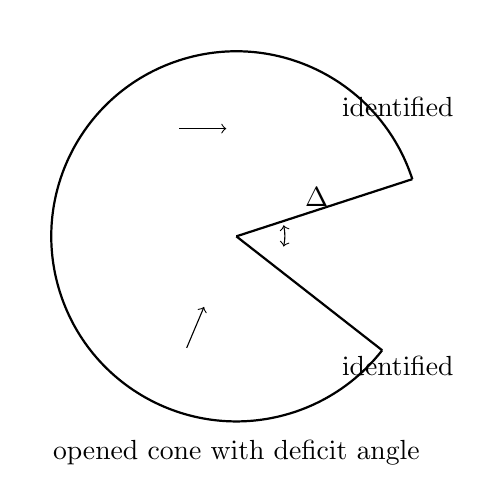
\begin{tikzpicture}[scale=1.0]
\draw[thick] (0,0) -- (18:2.35);
\draw[thick] (0,0) -- (322:2.35);
\draw[thick] (18:2.35) arc (18:322:2.35);
\draw[<->] (0.60,0.14) arc (13:-13:0.60);
\node at (1.02,0.50) {$\Delta$};
\draw[->] (118:1.55) -- ++(0.60,0.00);
\draw[->] (246:1.55) -- ++(0.22,0.52);
\node at (2.05,1.65) {identified};
\node at (2.05,-1.65) {identified};
\node at (0,-2.75) {opened cone with deficit angle};
\end{tikzpicture}
\caption{Schematic reconstruction of the conical-deficit argument. Flattening the cone requires cutting out a wedge; when the edges are reidentified, a transported vector fails to come back with the same direction.}
\end{figure}

Now imagine a vector field that is constant on the opened flat sheet. When we glue the sheet into a cone, that same ``constant'' transport around the tip produces a jump in direction. The vector comes back rotated. That is the effect of curvature in geometric form.

The lecture then translates this into the language we have built. We transport the vector so that its covariant derivative along the path is zero. Even so, when the path closes around a region of curvature, the vector fails to return to itself. That failure is the invariant content.

There is a second and more algebraic way to say the same thing, and Susskind says it is the more useful one. Take a vector field and differentiate it first in the \(r\)-direction and then in the \(s\)-direction. Compare that with differentiating first in the \(s\)-direction and then in the \(r\)-direction. In flat space the two operations agree. In curved space they do not. Their difference is essentially what one gets by taking the vector around a small closed loop.

\begin{figure}[h]
\centering
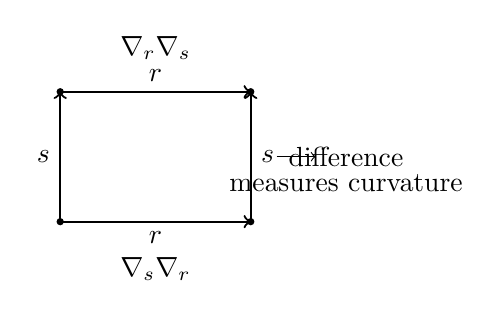
\begin{tikzpicture}[scale=1.1]
\fill (0,0) circle (1.2pt);
\fill (2.2,0) circle (1.2pt);
\fill (0,1.5) circle (1.2pt);
\fill (2.2,1.5) circle (1.2pt);
\draw[->,thick] (0,0) -- (2.2,0) node[midway,below] {$r$};
\draw[->,thick] (2.2,0) -- (2.2,1.5) node[midway,right] {$s$};
\draw[->,thick] (0,0) -- (0,1.5) node[midway,left] {$s$};
\draw[->,thick] (0,1.5) -- (2.2,1.5) node[midway,above] {$r$};
\node at (1.1,-0.55) {$\nabla_s\nabla_r$};
\node at (1.1,2.0) {$\nabla_r\nabla_s$};
\node at (3.3,0.75) {difference};
\node at (3.3,0.45) {measures curvature};
\draw[->] (2.5,0.75) -- (2.95,0.75);
\end{tikzpicture}
\caption{A small-loop version of the lecture's commutator argument. The two orders of covariant differentiation correspond to the two ways of going around the loop.}
\end{figure}

At this point Susskind does something pedagogically sensible. He does not grind through the entire double covariant derivative on the board. He says the calculation is mechanical, tells the class to do the plug-in themselves, and gives the answer. One computes \(\nabla_s\nabla_r V_n\), computes \(\nabla_r\nabla_s V_n\), subtracts, and defines the coefficient of \(V_t\) to be the curvature tensor:
\begin{equation}
(\nabla_s\nabla_r-\nabla_r\nabla_s)V_n
=
R^{t}{}_{nrs}V_t.
\end{equation}
In canonical Levi-Civita form,
\begin{equation}
R^{t}{}_{nrs}
=
\partial_r\Gamma^{t}{}_{sn}
-
\partial_s\Gamma^{t}{}_{rn}
+
\Gamma^{p}{}_{sn}\Gamma^{t}{}_{rp}
-
\Gamma^{p}{}_{rn}\Gamma^{t}{}_{sp}.
\end{equation}
This is the Riemann curvature tensor.

The lecture's emphasis is not on memorizing the precise index pattern of the formula, but on seeing what sort of object it is. There are two terms involving derivatives of Christoffel symbols and two terms involving products of Christoffel symbols. Since \(\Gamma\) itself is built from first derivatives of the metric, the first two terms in \(R\) contain second derivatives of \(g\), while the last two contain quadratic combinations of first derivatives. That is exactly what we should have expected. First derivatives of the metric can be made to vanish at a point by Gaussian normal coordinates; second derivatives cannot, in general. So the curvature tensor probes precisely what local flattening cannot erase.

This gives the promised diagnostic. If the curvature tensor vanishes everywhere, the space is flat. If it is nonzero anywhere, there is genuine curvature. That is still a pointwise calculation, and if the metric were given only numerically one would still have to check point by point. But it is incomparably better than searching through all coordinate systems. If the metric is given analytically, one differentiates, constructs \(R\), and checks whether the analytic result vanishes.

\subsection{Question \& Answer}

\paragraph{Question.} What distinguishes a real gravitational field from acceleration?

\paragraph{Answer.} Tidal forces. An accelerated coordinate system can imitate many features of gravity, but it cannot produce the genuine relative stretching and squeezing that comes from curvature. A real gravitational field produced by real matter varies from place to place, and that variation shows up as tidal distortion. The curvature tensor is the local invariant measure of that effect.

Susskind makes this physical identification with some insistence. If a very small body falls in a gravitational field, it may experience almost no noticeable tidal effect, because the field hardly changes across its size. A sufficiently large body in the same environment will be stretched and compressed, because different parts of it sample different local geometry. The correspondence with curvature is exact, not accidental. In this sense curvature is what gravity becomes when one strips away the coordinate language and asks for the local invariant content.

He also adds a useful caution. A truly uniform gravitational field does not occur as a real exact field produced by matter. One may approximate the Earth's field as uniform over a sufficiently small region, and then a freely falling observer feels essentially nothing. That is precisely because tidal forces are small there. But when the field varies appreciably across an object, curvature announces itself by deformation.

So the lecture ends where it promised to end. We began by asking how to distinguish genuine geometry from funny coordinates. We then found that local flatness can always be arranged at first order, that naive differentiation fails because coordinate frames themselves change, that the covariant derivative repairs the failure, and that curvature finally appears in the noncommutation of covariant derivatives or, geometrically, in transporting a vector around a loop.

\section{Summary}

This chapter follows the lecture's arc from notation to invariant content. The metric defines lengths, has an inverse, is positive definite in the Riemannian setting, and raises and lowers indices. At a chosen point we may always introduce Gaussian normal coordinates so that the metric looks flat and its first derivatives vanish. That local flattening, however, immediately tells us that ordinary derivatives of vector components cannot be tensorial. The covariant derivative repairs the problem by subtracting off the variation of the coordinates themselves, and the Christoffel symbols are the coefficients that carry that coordinate dependence.

But Christoffel symbols are not yet curvature. Curvature appears only when we compare two successive covariant differentiations in opposite orders, or geometrically when we transport a vector around a closed loop and fail to come back to what we started with. The resulting Riemann tensor is the diagnostic quantity the lecture set out to find. It vanishes in flat space and becomes nonzero precisely when there is real geometric content left over after all coordinate tricks have been exhausted. In the next lecture that same content will be reinterpreted directly as gravity, with the transition from Riemannian to Einsteinian geometry and then the Schwarzschild example; geodesics, which were postponed here, will re-enter there.